% Chapter Template

\chapter{Inferrable Languages} % Main chapter title

\label{ChapterX} % Change X to a consecutive number; for referencing this chapter elsewhere, use \ref{ChapterX}

%----------------------------------------------------------------------------------------
%	SECTION 1
%----------------------------------------------------------------------------------------

\section{Introduction}

The concept of statistics and blackboxes has been drawn out extensively in theories and applications for decades but what of languages and knowing what word can be used to generate the next series of words? Everyone guesses what words can come out of someone talking given enough experience. In this article, the idea of inferrable languages is presented which are languages that allow the next series of words in the sequence to be inferred given enough samples in the sequence.


\section{Applying The Fibonnaci Decider}

Given the definition of the Fibonacci decider and a Lindenmayer system, insight can be derived from to that there exists the commutative and noncommutative properties of the operations.

$\\ $

$\textbf{Decider}$ for $x_1, y_1, z_1$

$-x_1 = y_1 - z_1$

$y_1 = -x_1 - z_1$

$-z_1 = x_1 - y_1$

$\\ $

$\textbf{Decider}$ for $x_2, y_2, z_2$

$x_2 = y_2 - z_2$

$-y_2 = x_2 - z_2$

$z_2 = x_2 - y_2$

$\\ $

$\textbf{Fibonacci Decider}$

$x_1 = -y_1 +z_2 - x_2 + y_2 - z_1$

$-y_1 = z_2 - x_2 + y_2 - z_1 + x_1$

$z_2 = -x_2 + y_2 - z_1 + x_1 - y_1$

$-x_2 = y_2 - z_1 + x_1 - y_1 + z2$

$y_2 = -z_1 + x_1 - y_1 + z_2 - x_2$

$-z_1 = x_1 - y_1 + z_2 - x_2 + y_2$

$\\ $

$\textbf{Lindenmayer System}$

L is the definition of the D0L System

$L = (V,\omega,P)$

V are the characters in the language called the alphabet

$\omega$ is the starting string called the start

P are the production rules in the language called the rules

$\\ $

$\textit{alphabet}$. $= \{a,b\}$

$\textit{rules}$. $= \{a \Rightarrow ab, b \Rightarrow a\}$

$\textit{start}$. $= b$

$\\ $

\section{Fibonacci DOL Decider Left Hand Side}

Representing the left hand side of the Fibonacci sequence as a D0L system alphabet requires an alphabet, rules, and a starting state.



$\\ $

The first six sequences in the 

$\\ $

$b\ a\ ab\ aba\ abaab\ abaababa\ abaababaabaab\ abaababaabaababaabaab$

$\\ $

The length are as follows.

$\\ $

$1\ 1\ 2\ 3\ 5\ 8\ 13\ 21$

$\\ $

Set them as variables in the decider as follows.

$\\ $

$\textbf{Decider}$ for $x_1, y_1, z_1$

$-x_1 = y_1 - z_1$

$y_1 = -x_1 - z_1$

$-z_1 = x_1 - y_1$

$\\ $

$\textbf{Decider}$ for $x_2, y_2, z_2$

$x_2 = y_2 - z_2$

$-y_2 = x_2 - z_2$

$z_2 = x_2 - y_2$

$\\ $

$z_2 = b$

$y_2 = a$

$x_2 = ab$

$z_1 = aba$

$y_1 = abaab$

$x_1 = abaababa$

$\\ $

$\textbf{Decider}$ for $x_1, y_1, z_1$

$\\ $

$\textit{\textbf{-x\textsubscript{1} = y\textsubscript{1} - z\textsubscript{1}}}$

$\textit{\textbf{- abaababa = abaab - aba}}$

$-abaababa + aba = abaab$

$-abaababa - abaab = -aba$

$\\ $

$\textbf{y\textsubscript{1} = -x\textsubscript{1} - z\textsubscript{1}}$

$\textbf{abaab = - abaababa - aba}$

abaab + abaababa = - aba

abaab + aba = - abaababa

$\\ $

$\textbf{-z\textsubscript{1} = x\textsubscript{1} - y\textsubscript{1}}$

$\textbf{- aba = abaababa - abaab}$

- aba + abaab = abaababa 

- aba - abaababa = - abaab

$\\ $

$\textbf{Decider}$ for $x_2, y_2, z_2$

$\textbf{x\textsubscript{2} = y\textsubscript{2} - z\textsubscript{2}}$

$ab - b = a$

$ab - a = b$

$\\ $

$\textbf{-y\textsubscript{2} = x\textsubscript{2} - z\textsubscript{2}}$

-a + b = ab

-a - ab = -b

$\\ $

$\textbf{z\textsubscript{2} = x\textsubscript{2} - y\textsubscript{2}}$

b - ab = -a

b + a = ab

$\\ $

Generalized equations for $x_1, y_1, z_1$

$\\ $

$\textit{\textbf{-a = b - c}}$

$-a + c = b$

$-a - b = - c$

$\\ $

$\textbf{b = -a - c}$

b + a = -c

b + c = a

$\\ $

$\textbf{-c = a - b}$

-c + b = a

-c - a = -b

$\\ $

Generalized equations for $x_2, y_2, z_2$

$\\ $

$\textit{\textbf{a = b + c}}$

$a - c = b$

$a - b = c$

$\\ $

$\textbf{b = a - c}$

b - a = -c

b + c = a

$\\ $

$\textbf{-c = a - b}$

-c + b = a

-c - a = -b

$\\ $

\section{Fibonacci DOL Decider Right Hand Side}

$\textbf{Fibonacci Decider}$

$x_1 = -y_1 +z_2 - x_2 + y_2 - z_1$

$-y_1 = z_2 - x_2 + y_2 - z_1 + x_1$

$z_2 = -x_2 + y_2 - z_1 + x_1 - y_1$

$-x_2 = y_2 - z_1 + x_1 - y_1 + z2$

$y_2 = -z_1 + x_1 - y_1 + z_2 - x_2$

$-z_1 = x_1 - y_1 + z_2 - x_2 + y_2$

$\\ $

$
\begin{matrix}
 \textbf{abaababa = -abaab + b - ab + a -aba}\\
abaababa - b + ab - a + aba = -abaab \\
abaababa + abaab + ab - a + aba = b \\
abaababa + abaab - b - a + aba = -ab \\
abaababa + abaab - b + ab + aba = a \\
abaababa + abaab - b + ab - a = -aba \\
\end{matrix}
$

$\\ $

$
\begin{matrix}
 \textbf{-abaab = b - ab + a -aba + abaababa}\\
-abaab + ab - a + aba - abaababa = b \\
-abaab - b - a + aba - abaababa = -ab \\
-abaab - b + ab + aba - abaababa = a\\
-abaab - b + ab - a - abaababa = -aba\\
-abaab - b + ab - a + aba = abaababa \\
\end{matrix}
$

$\\ $

$
\begin{matrix}
 \textbf{b = -ab + a - aba + abaababa - abaab}\\
b - a + aba - abaababa + abaab = -ab \\
b + ab + aba - abaababa + abaab = a \\
b + ab + aba - abaababa + abaab = -aba\\
b - ab + a -aba + abaab = abaababa\\
b - ab - a + aba - abaababa = -abaab \\
\end{matrix}
$

$\\ $

$
\begin{matrix}
 \textbf{-ab = a - aba + abaababa - abaab + b}\\
- ab + aba - abaababa + abaab - b = a \\
- ab - a - abaababa + abaab -b = - aba \\
- ab - a + aba + abaab - b = abaababa\\
- ab -a + aba - abaababa - b = -abaab\\
-ab - a + aba -  abaababa + abaab = b\\
\end{matrix}
$

$\\ $

$
\begin{matrix}
 \textbf{a = aba + abaababa - abaab + b - ab}\\
a + abaababa - abaab + b - ab = aba \\
a - aba - abaab + b - ab = -abaababa \\
a - aba + abaababa + b - ab = abaab\\
a - aba + abaababa - abaab - ab = -b\\
a - aba + abaababa - abaab + b = ab\\
\end{matrix}
$

$\\ $

$
\begin{matrix}
 \textbf{-aba = abaababa - abaab + b - ab + a}\\
- aba + abaab - b + ab - a = abaababa \\
-aba - abaababa - b + ab + a = -abaab \\
-aba - abaababa + abaab + ab - a = b\\
-aba - abaababa + abaab - b - a = -ab\\
-aba - abaababa + abaab - b + ab = a\\
\end{matrix}
$

\section{The Law of Commutativity and Noncommutativity}

The law of commutativity and the law of noncommutativity combined gives the law of commutativity and noncommutativity

$\\ $
 
The Law of Commutativity

a + b = b + a

ex. 8 + 5 = 5 + 8

$\\ $

The Law of Noncommutativity

a+ b != b + a

ex. 8 - 5 != 5 - 8

$\\ $

Each equation in the example on the left has permutations.

From this example, it can be implied that for every variable, n, in an equation there is $n^2$ permutations in the sequence.

The first equation is bold and italicized in the set to make a decider.



$
\begin{matrix}
 \textit{\textbf{a = b + c}} & \textbf{b = a - c} & \textbf{-c = a - b}\\
 b = a - c & b - a = -c & -c + b = a\\
 -c = a - b & b + c = a & -c - a = -b
\end{matrix}
$

\section{Operations}

Operations for the right hand side (RHS) versus the left hand side (LHS) represents different operations of the string in different scenarios.

$\\ $

RHS Evaluation

Right to Left

+ Remove from the back

- Add to the front

abaababa = - abaab + b - ab + a -aba

abaababa = - abaab + b - ab -ab

abaababa = - abaab + b - abab

abaababa = - abaab - aba

abaababa = - abaababa

$\\ $

LHS Evaluation

Left to Right

+ Remove at the front

- Add to the back

abaababa + abaab - b + ab - a = -aba

aba - b + ab - a = -aba

abab + ab - a = -aba

ab - a = -aba

aba = -aba

$\\ $

$\textit{Proposition.}$The characteristic series of a rational cyclic language is a Z-linear combination of characters of finite deterministic automata.

$\\ $

\section{Definition Of Support}

A support is defined as the following:

A* is a word

S is the function

Image by S of a word w is denoted by (S,w) and is the coefficient of w in S

Support(S) = {w in A* such that (S,w) != 0}

$\\ $

Now we take deciders of a monomial and the picking function to redefine the support of a noncommutative rational language

R is the rational numbers where x in R = a/b

such that a,b is in integers and b $\neq$ 0

Q is the quotient space represented in topology such that A/~ where are sets and ~ is the divisions of A

R-rational is the representation of R as the polynomial function

Q-rational is the representation of Q as a polynomial

\section{Rationals Of Picking Function}

Support of the Fibonacci Picking Function of the deciders of a monomial.

Q-rational-deciders are the possible monomial deciders of Q-rational-string. Use the picking function, PF, to choose one decision function in Q-rational-deciders, we see a mapping from Q-rational => R-rational.

\begin{figure}[H]
  \centering
  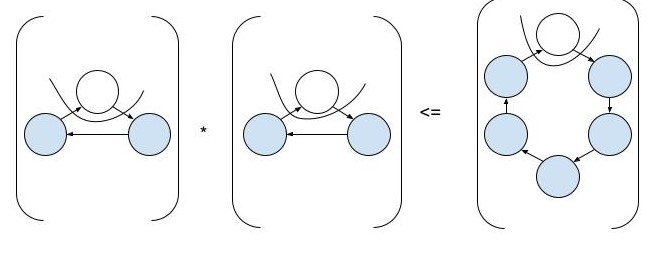
\includegraphics[scale=1]{0219Rationals.jpg}
  \caption{Q rational image of the q rational string, $x^3/3$, $x^3/3$, and $X^6/x$.}
  \label{fig:0219Rationals}
\end{figure}

Deciders for $x^3/x$ has 9 possible configurations, or, in algebraic terms, permutations, and $x^6/x$ has 36 possible configurations. This equates to R rational for $x^3/x$ being $1/9$ and $x^6/x$ being $1/36$.

This implies the existence of the map between Q rational to R rational.

\section{Support Of Picking Function}

The support of an inferrable language is now defined to be:

$\\ $

Dupport of PF of Q-rational-deciders = support(PF(Q-rational-deciders))

$\\ $

Decider in Q-rational-deciders such that decider is unique $\equiv$ Determinant of a configuration of a decider != 0

$\\ $

The decider chosen has an equation that is bold and italicized and there is a set of equations that are distinctly bold and italic that complete this equation to form the decider.

\section{Law Of Strings}

Although the law of commutativity and noncommutativity is a theorem, it's helpful to get a big picture view. Let's condense the law of commutativity and noncommutativity down even further to find some laws.

This is operating on variables, strings, and representations of it.

\section{Commutativity Of Addition}

Take the length function, length(s) $\equiv$ l(s), and apply to the '=' addition operations and see it's equivalence. Set b to a and reversal is accomplished.

\section{Commutativity Of Multiplication}

Commutativity of Multiplication

\section{Additive Identity}

The LHS and RHS are equations that test whether or not they are true or false, or in terms of computational complexity theory, it is satisfiable.
10 = 10 evaluates to true or 1.
01 != 10 evaluates to true or 1 too.

\section{Multiplicative Identity}

The Identity of Itself on Multiplication

\section{Additive Inverse}

The Additive Inverse

General Equivalence

Commutativity under Equivalence

General Reversal

Commutativity under reversal

\section{Multiplicative Inverse}

Given a monomial such that it represents a monomial in a polynomial, if we loop around once, we see the identity path.

\section{Generalized Operations}

The set of images that describes the operations on monomials can be put together to find a 2x2 matrix that describes them using the laws provided.

\section{Generalized Communativity}

For showing commutativity, have the following images to represent addition and multiplication.

\section{Associativity Of Addition}

Associativity of addition is defined as:

a + (b + c) = (a + b) + c

\section{Associativity Of Multiplication}

Associativity of multiplication is defined as:

a * (b*c) = (a*b)*c

\section{Distibutivity}

Distributivity is defined as:

a*(b+c) = a*b + a*c

\section{Field}

The Field Axioms are defined as:

